\section{Inside Git}
\subsection{Objekte}
\begin{frame}{Objekte}
    \begin{itemize}
        \item Git als map-type storage
        \item Hashes bilden auf Daten ab
        \item Speicherung in einzelnen Dateien (``der Kernel macht das'')
        \item jedes Objekt in git ist eine solche Datei, jeweils ein ``Snapshot''
            einer Version
            \begin{itemize}
                \item \emph{blob} für Dateien
                \item \emph{tree} für Verzeichnisse\\
                    $\rightarrow$ Referenzen auf einzelne \emph{blobs} + Metadaten
                \item \emph{commit} für das ganze Repository\\
                    $\rightarrow$ Wurzelverzeichnis als \emph{tree} + Metadaten
            \end{itemize}
        \item \emph{tree} und \emph{commit} enthalten Informationen in Klartext,  \emph{blob} den Dateiinhalt
    \end{itemize}

    \pause
    \vspace{0.5em}
    \makebox[\textwidth][c]{
        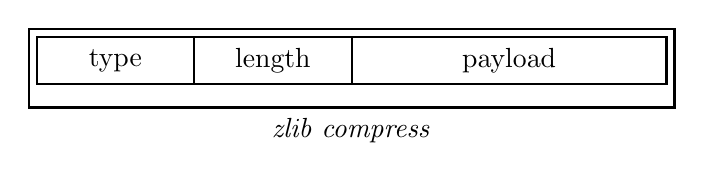
\begin{tikzpicture}[x=1cm,y=1cm]
            \node (rect) at (0, 0) [draw,thick,minimum width=2cm,minimum height=0.6cm] {type};
            \node (rect) at (2, 0) [draw,thick,minimum width=2cm,minimum height=0.6cm] {length};
            \node (rect) at (5, 0) [draw,thick,minimum width=4cm,minimum height=0.6cm] {payload};
            \node (rect) at (3, -0.1) [draw,thick,minimum width=8.2cm,minimum height=1cm,label=below:\emph{zlib compress}] {};
        \end{tikzpicture}
    }
\end{frame}

\subsection{Working copy}
\begin{frame}{Working copy}
    \begin{itemize}
        \item In \texttt{.git/} liegen alle Objekte, mit Hashes als Dateinamen
        \item Wie soll man damit arbeiten?
        \item $\rightarrow$ aktuelle Version (\emph{HEAD}) liegt im Hauptverzeichnis
        \item verständliche Dateinamen (statt Hashes)
        %\item wechseln der Version per \textsc{checkout}
        %    \bash{git checkout 4b5c8e2f95a4407c4d0c596565b367eaca07af57}
        %    $\rightarrow$ nicht möglich, wenn unversionierte Änderungen vorliegen
    \end{itemize}
\end{frame}

\begin{frame}{Der Index (Staging Area)}
    \begin{itemize}
        \item ``Laderampe''
        \item erst wählen, welche Änderungen übernommen werden sollen (\emph{add})
        \item dann diese Änderungen speichern (\emph{commit})
    \end{itemize}

\end{frame}

\subsection{Vom Leben einer Datei}
\begin{frame}[label=life]{Vom Leben einer Datei}
    \tikzset{
        state/.style = {
            rectangle,
            minimum width=2cm,
            minimum height=1cm,
            draw=black,
            thick,
            rounded corners=3pt,
            font=\small,
            align=center
        },
        arrow/.style = {
            draw,
            thick,
            -latex,
        }
    }

    \vspace{1cm}
    \makebox[\textwidth][c]{
        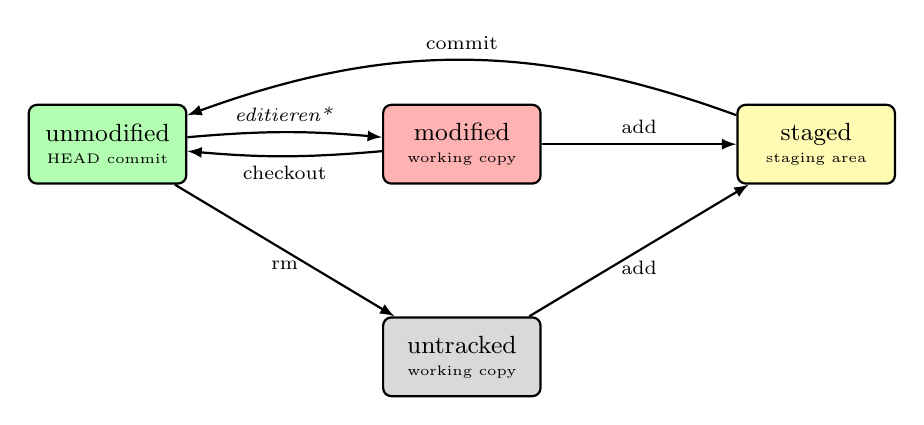
\begin{tikzpicture}[x=0.9cm,y=0.9cm]
            \node[state,fill=green!30!white] (unmodified) at (-5, 0) {unmodified\\[-3pt]\tiny HEAD commit};
            \node[state,fill=red!30!white] (modified) at (0, 0) {modified\\[-3pt]\tiny working copy};
            \node[state,fill=yellow!30!white] (staged) at (5, 0) {staged\\[-3pt]\tiny staging area};
            \node[state,fill=gray!30!white] (untracked) at (0, -3) {untracked\\[-3pt]\tiny working copy};

            \draw[arrow] (unmodified) to[bend left=5] node[midway,above] {\scriptsize\emph{editieren*}} (modified);
            \draw[arrow] (modified) to[bend left=5] node[midway,below] {\scriptsize checkout} (unmodified);
            \draw[arrow] (modified) to node[midway,above] {\scriptsize add} (staged);
            \draw[arrow] (staged) to[bend right=20] node[midway,above] {\scriptsize commit} (unmodified);
            \draw[arrow] (untracked) to node[midway,below] {\scriptsize add} (staged);
            \draw[arrow] (unmodified) to node[midway,below] {\scriptsize rm} (untracked);
        \end{tikzpicture}
    }
\end{frame}
